\documentclass[11pt]{article}
\usepackage[margin=1in]{geometry}
\usepackage{graphicx}
\usepackage{enumitem}
\usepackage[T1]{fontenc}
\usepackage[utf8]{inputenc}

% Toggle this to show/hide correct answers in the output.
\newif\ifshowanswers
\showanswerstrue

\begin{document}

\begin{center}
{\LARGE OOP Course Quiz}\\
\vspace{0.25em}
{\normalsize Assessment covering class diagrams, design patterns, sequence diagrams, and use case diagrams.}
\end{center}

\vspace{1em}
\begin{enumerate}[leftmargin=*, label=\textbf{\arabic*.}]

\item
Review the diagram below.
\begin{center}
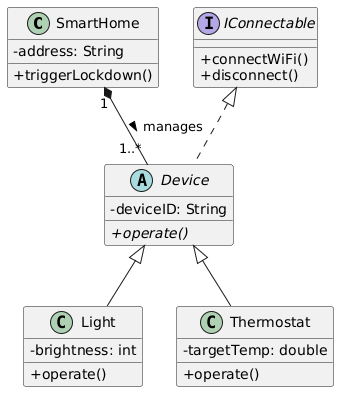
\includegraphics[width=0.85\linewidth]{d1.png}
\\{\small Diagram 1}
\end{center}
What type of relationship is represented by the solid diamond between SmartHome and Device?
\begin{enumerate}[label=\alph*)]
\item Aggregation
\item \ifshowanswers\textbf{Composition}\else Composition\fi
\item Generalization
\item Association
\end{enumerate}

\item
Review the diagram below.
\begin{center}
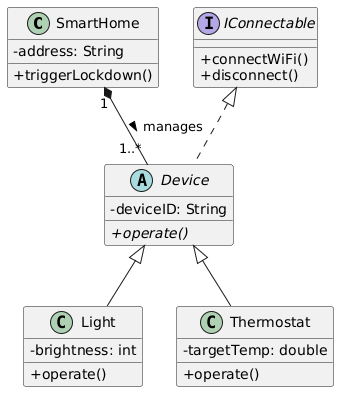
\includegraphics[width=0.85\linewidth]{d1.png}
\\{\small Diagram 1}
\end{center}
Why is the \texttt{Device} class marked as abstract?
\begin{enumerate}[label=\alph*)]
\item It contains only private methods.
\item \ifshowanswers\textbf{It is a base class that cannot be directly instantiated, requiring subclasses to define specific behaviors.}\else It is a base class that cannot be directly instantiated, requiring subclasses to define specific behaviors.\fi
\item It prevents the class from having any attributes.
\item It allows the class to inherit from multiple interfaces.
\end{enumerate}

\item
Review the diagram below.
\begin{center}
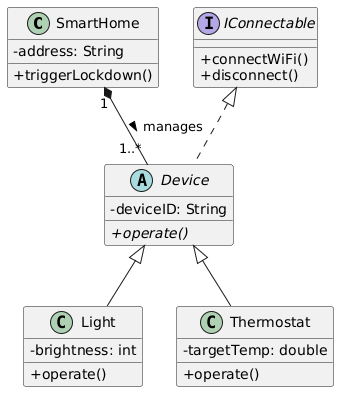
\includegraphics[width=0.85\linewidth]{d1.png}
\\{\small Diagram 1}
\end{center}
What does the multiplicity "1..*" next to the Device class indicate?
\begin{enumerate}[label=\alph*)]
\item A SmartHome can have exactly one Device.
\item \ifshowanswers\textbf{A SmartHome must contain at least one Device, but can contain many.}\else A SmartHome must contain at least one Device, but can contain many.\fi
\item A Device can belong to multiple SmartHomes.
\item A SmartHome can exist with zero Devices.
\end{enumerate}

\item
Review the diagram below.
\begin{center}
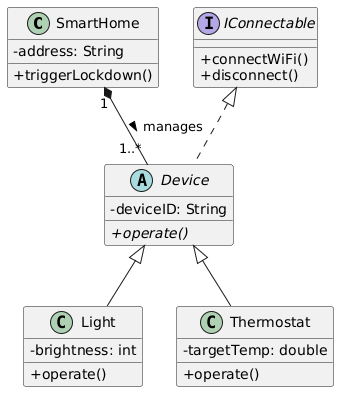
\includegraphics[width=0.85\linewidth]{d1.png}
\\{\small Diagram 1}
\end{center}
Because the \texttt{Device} class implements the \texttt{IConnectable} interface, what is required of the \texttt{Light} class?
\begin{enumerate}[label=\alph*)]
\item It must create its own separate interface.
\item It can choose whether or not to include networking methods.
\item \ifshowanswers\textbf{It inherits the interface contract and must have implementations for the \texttt{connectWiFi()} and \texttt{disconnect()} methods.}\else It inherits the interface contract and must have implementations for the \texttt{connectWiFi()} and \texttt{disconnect()} methods.\fi
\item It must override the \texttt{SmartHome} attributes.
\end{enumerate}

\item
Review the diagram below.
\begin{center}
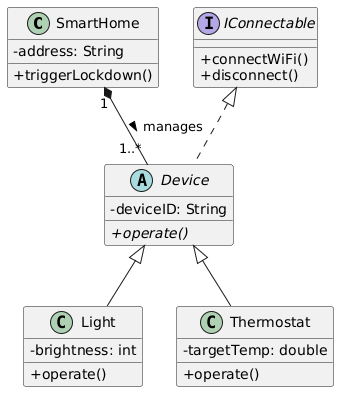
\includegraphics[width=0.85\linewidth]{d1.png}
\\{\small Diagram 1}
\end{center}
If a program calls the \texttt{operate()} method on a \texttt{Device} variable that currently holds a \texttt{Thermostat} object, which concept ensures the \texttt{Thermostat}'s specific version of the method runs?
\begin{enumerate}[label=\alph*)]
\item \ifshowanswers\textbf{Polymorphism}\else Polymorphism\fi
\item Encapsulation
\item Method Overloading
\item Multiple Inheritance
\end{enumerate}

\item
Review the diagram below.
\begin{center}
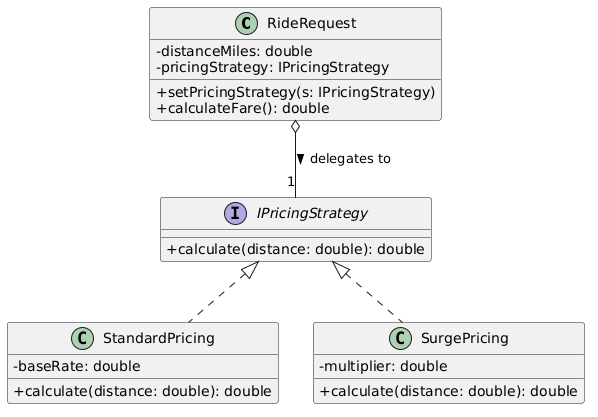
\includegraphics[width=0.85\linewidth]{d2.png}
\\{\small Diagram 2}
\end{center}
What is the primary benefit of delegating the fare calculation to the \texttt{IPricingStrategy} interface?
\begin{enumerate}[label=\alph*)]
\item It makes the code run faster.
\item \ifshowanswers\textbf{It allows new pricing algorithms to be added without modifying the \texttt{RideRequest} class.}\else It allows new pricing algorithms to be added without modifying the \texttt{RideRequest} class.\fi
\item It allows \texttt{RideRequest} to inherit from multiple classes.
\item It hides the distance variable from the user.
\end{enumerate}

\item
Review the diagram below.
\begin{center}
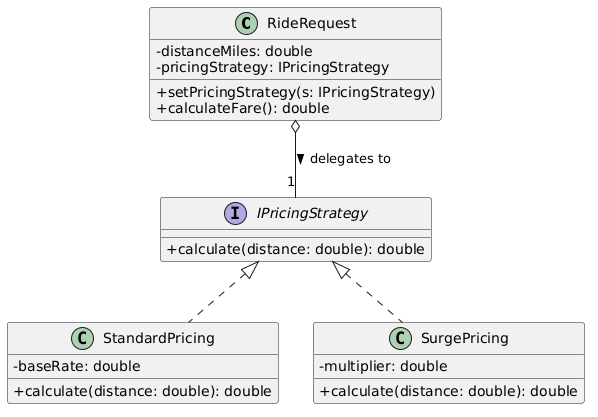
\includegraphics[width=0.85\linewidth]{d2.png}
\\{\small Diagram 2}
\end{center}
In this diagram, what exactly is \texttt{IPricingStrategy}?
\begin{enumerate}[label=\alph*)]
\item A concrete class that contains the math for calculating fares.
\item \ifshowanswers\textbf{An interface that acts as a blueprint, defining a method signature that other classes must implement.}\else An interface that acts as a blueprint, defining a method signature that other classes must implement.\fi
\item A subclass that inherits from \texttt{RideRequest}.
\item An external database that stores standard pricing rates.
\end{enumerate}

\item
Review the diagram below.
\begin{center}
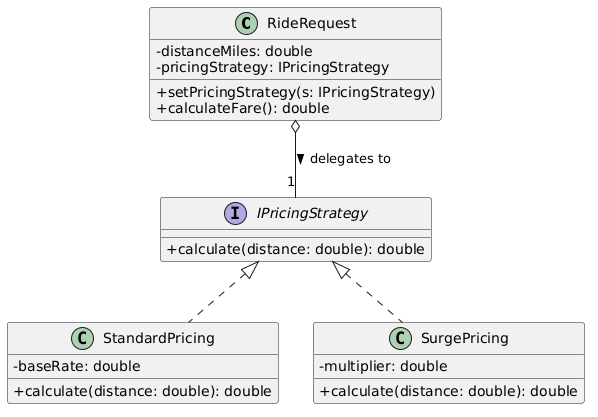
\includegraphics[width=0.85\linewidth]{d2.png}
\\{\small Diagram 2}
\end{center}
What does the empty diamond arrow connecting \texttt{RideRequest} to \texttt{IPricingStrategy} represent?
\begin{enumerate}[label=\alph*)]
\item Inheritance
\item \ifshowanswers\textbf{Aggregation}\else Aggregation\fi
\item Composition
\item Realization
\end{enumerate}

\item
Review the diagram below.
\begin{center}
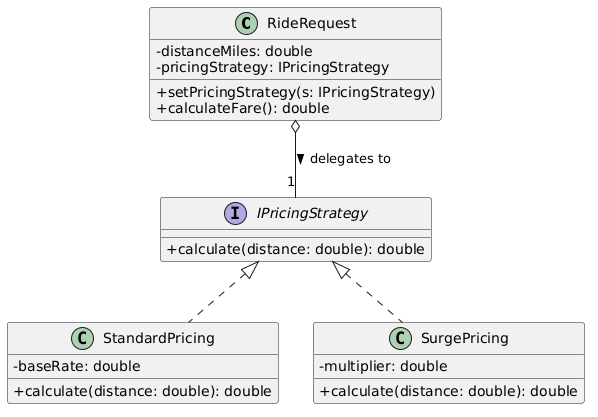
\includegraphics[width=0.85\linewidth]{d2.png}
\\{\small Diagram 2}
\end{center}
When the \texttt{RideRequest} class executes the \texttt{calculate()} method, how does the program know whether to use the math from \texttt{StandardPricing} or \texttt{SurgePricing}?
\begin{enumerate}[label=\alph*)]
\item The \texttt{RideRequest} class contains an internal if/else statement to decide.
\item It runs both methods and adds the results together.
\item \ifshowanswers\textbf{It executes the method belonging to the specific object type (Standard or Surge) that is currently assigned to the \texttt{pricingStrategy} variable.}\else It executes the method belonging to the specific object type (Standard or Surge) that is currently assigned to the \texttt{pricingStrategy} variable.\fi
\item The interface calculates it automatically.
\end{enumerate}

\item
Review the diagram below.
\begin{center}
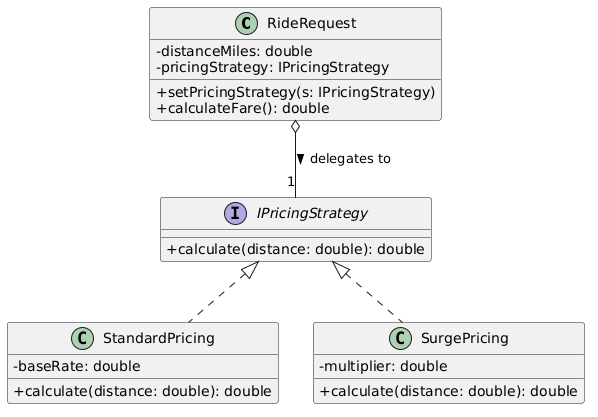
\includegraphics[width=0.85\linewidth]{d2.png}
\\{\small Diagram 2}
\end{center}
How would you add a \texttt{HolidayPricing} calculation to this system?
\begin{enumerate}[label=\alph*)]
\item Add a new \texttt{if/else} statement inside \texttt{RideRequest}.
\item Modify the \texttt{StandardPricing} class to include holiday logic.
\item Change \texttt{IPricingStrategy} into an abstract class.
\item \ifshowanswers\textbf{Create a new \texttt{HolidayPricing} class that implements \texttt{IPricingStrategy}.}\else Create a new \texttt{HolidayPricing} class that implements \texttt{IPricingStrategy}.\fi
\end{enumerate}

\item
Review the diagram below.
\begin{center}
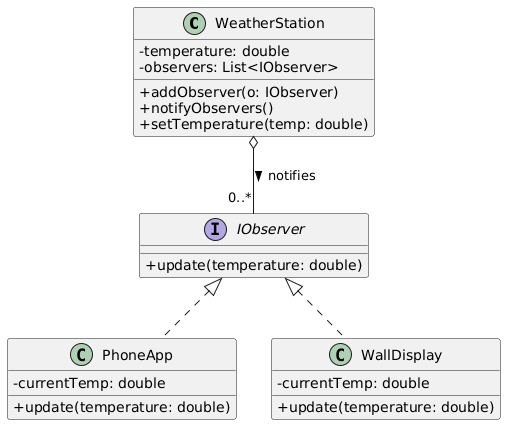
\includegraphics[width=0.85\linewidth]{d3.png}
\\{\small Diagram 3}
\end{center}
According to the diagram, what type of data is stored in the \texttt{observers} attribute of the \texttt{WeatherStation} class?
\begin{enumerate}[label=\alph*)]
\item A list of temperature values.
\item A single \texttt{PhoneApp} object.
\item \ifshowanswers\textbf{A list of objects, as long as those objects implement the \texttt{IObserver} interface.}\else A list of objects, as long as those objects implement the \texttt{IObserver} interface.\fi
\item A list of strings containing weather forecasts.
\end{enumerate}

\item
Review the diagram below.
\begin{center}
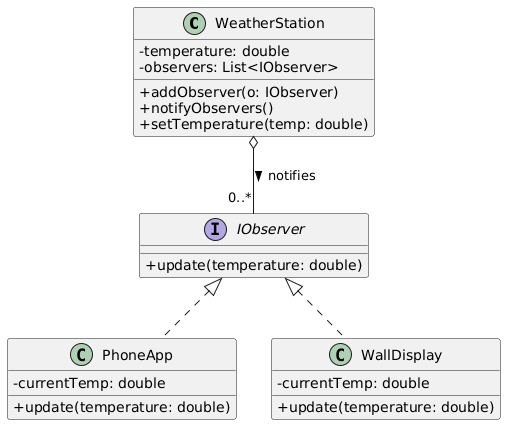
\includegraphics[width=0.85\linewidth]{d3.png}
\\{\small Diagram 3}
\end{center}
Both \texttt{PhoneApp} and \texttt{WallDisplay} contain an \texttt{update(temperature: double)} method. Why is this required by the architecture?
\begin{enumerate}[label=\alph*)]
\item They inherit the method directly from the \texttt{WeatherStation} class.
\item It is a coincidence that they share the same method name.
\item \ifshowanswers\textbf{They both implement the \texttt{IObserver} interface, which forces them to define their own version of this method.}\else They both implement the \texttt{IObserver} interface, which forces them to define their own version of this method.\fi
\item \texttt{PhoneApp} is a parent class to \texttt{WallDisplay}.
\end{enumerate}

\item
Review the diagram below.
\begin{center}
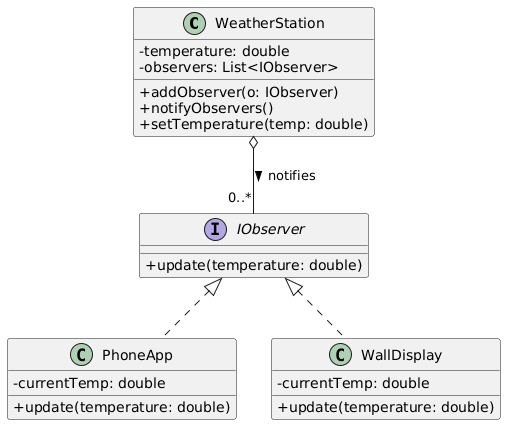
\includegraphics[width=0.85\linewidth]{d3.png}
\\{\small Diagram 3}
\end{center}
Why does the \texttt{WeatherStation} maintain a list of \texttt{IObserver} interfaces rather than concrete classes like \texttt{PhoneApp}?
\begin{enumerate}[label=\alph*)]
\item Because interfaces use less memory.
\item \ifshowanswers\textbf{To reduce coupling, allowing the station to notify any object that implements the interface without knowing its specific type.}\else To reduce coupling, allowing the station to notify any object that implements the interface without knowing its specific type.\fi
\item Because Java and C++ require lists to hold interfaces.
\item To prevent the observers from modifying the temperature.
\end{enumerate}

\item
Review the diagram below.
\begin{center}
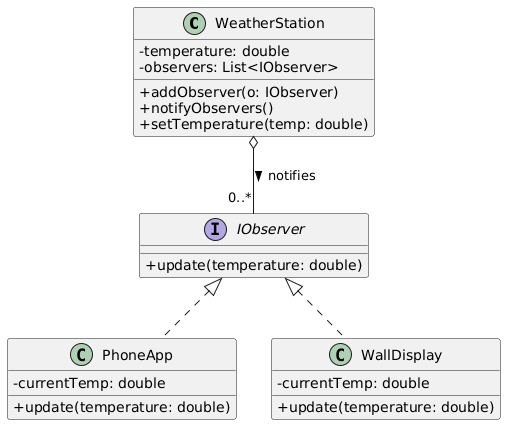
\includegraphics[width=0.85\linewidth]{d3.png}
\\{\small Diagram 3}
\end{center}
What does the dashed line with the unfilled arrow pointing from \texttt{PhoneApp} to \texttt{IObserver} mean?
\begin{enumerate}[label=\alph*)]
\item \ifshowanswers\textbf{The class implements (realizes) the interface.}\else The class implements (realizes) the interface.\fi
\item The class inherits from another class.
\item The class contains the interface.
\item The class depends on the interface temporarily.
\end{enumerate}

\item
Review the diagram below.
\begin{center}
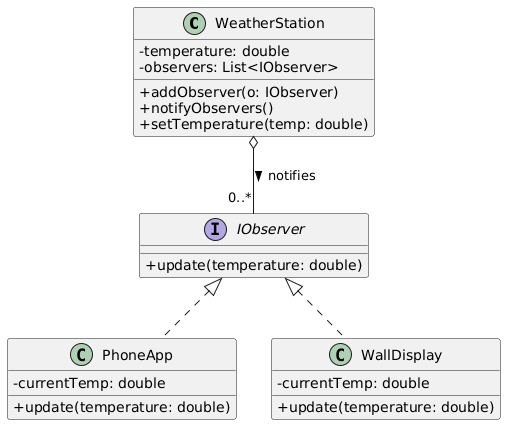
\includegraphics[width=0.85\linewidth]{d3.png}
\\{\small Diagram 3}
\end{center}
In the context of this pattern, the \texttt{WeatherStation} is typically referred to as the:
\begin{enumerate}[label=\alph*)]
\item Listener
\item Subscriber
\item \ifshowanswers\textbf{Subject}\else Subject\fi
\item Strategy
\end{enumerate}

\item
Review the diagram below.
\begin{center}
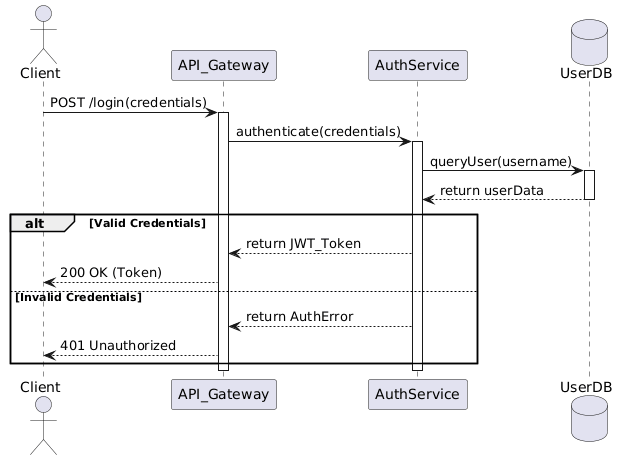
\includegraphics[width=0.85\linewidth]{d4.png}
\\{\small Diagram 4}
\end{center}
In a sequence diagram, what does a solid line with a solid arrowhead represent?
\begin{enumerate}[label=\alph*)]
\item \ifshowanswers\textbf{A synchronous message or method call}\else A synchronous message or method call\fi
\item An asynchronous message
\item A return message
\item An object creation
\end{enumerate}

\item
Review the diagram below.
\begin{center}
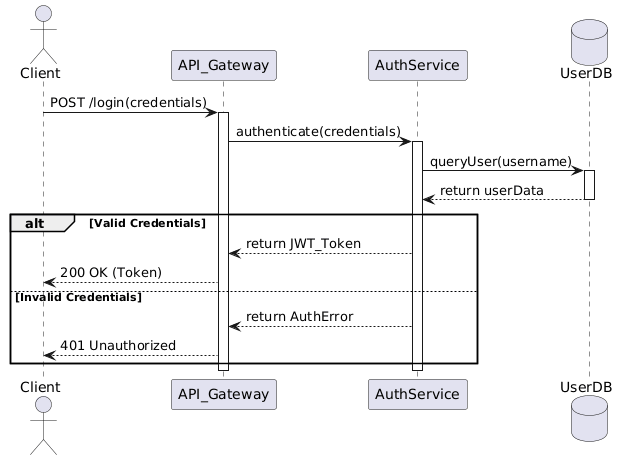
\includegraphics[width=0.85\linewidth]{d4.png}
\\{\small Diagram 4}
\end{center}
What do the vertical rectangular boxes on the lifelines indicate?
\begin{enumerate}[label=\alph*)]
\item The object is being created.
\item \ifshowanswers\textbf{The object is active and currently processing a method or task.}\else The object is active and currently processing a method or task.\fi
\item The object has been destroyed.
\item The object is waiting for user input.
\end{enumerate}

\item
Review the diagram below.
\begin{center}
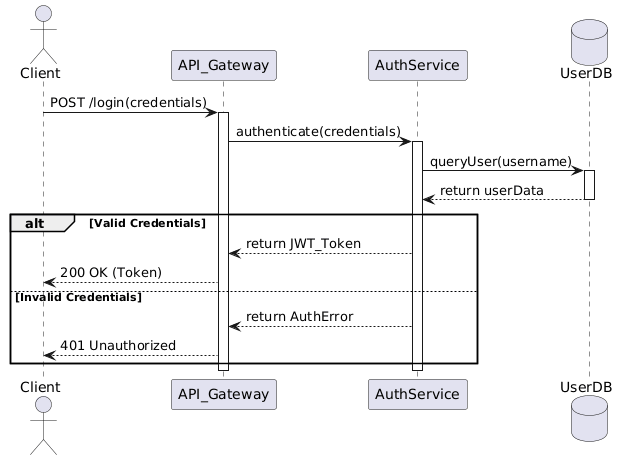
\includegraphics[width=0.85\linewidth]{d4.png}
\\{\small Diagram 4}
\end{center}
Reading the sequence diagram from top to bottom, what action happens immediately after the \texttt{AuthService} sends the \texttt{queryUser(username)} message to the \texttt{UserDB}?
\begin{enumerate}[label=\alph*)]
\item The \texttt{Client} logs in.
\item The \texttt{API\_Gateway} authenticates the user.
\item \ifshowanswers\textbf{The \texttt{UserDB} returns \texttt{userData} back to the \texttt{AuthService}.}\else The \texttt{UserDB} returns \texttt{userData} back to the \texttt{AuthService}.\fi
\item The \texttt{AuthService} returns a \texttt{JWT\_Token} to the \texttt{API\_Gateway}.
\end{enumerate}

\item
Review the diagram below.
\begin{center}
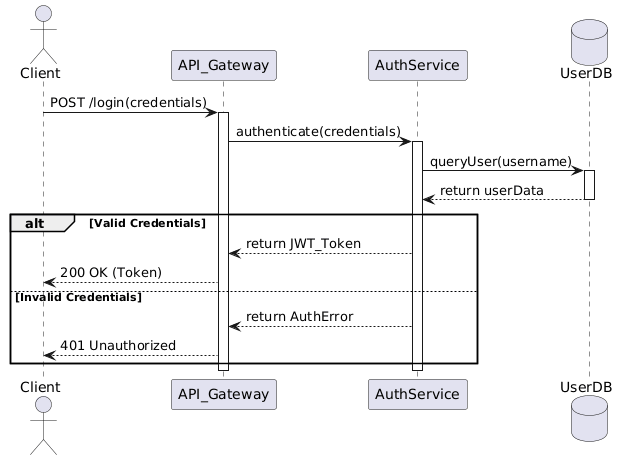
\includegraphics[width=0.85\linewidth]{d4.png}
\\{\small Diagram 4}
\end{center}
According to the diagram, which component is responsible for querying the \texttt{UserDB}?
\begin{enumerate}[label=\alph*)]
\item The Client
\item The API\_Gateway
\item \ifshowanswers\textbf{The AuthService}\else The AuthService\fi
\item The database queries itself
\end{enumerate}

\item
Review the diagram below.
\begin{center}
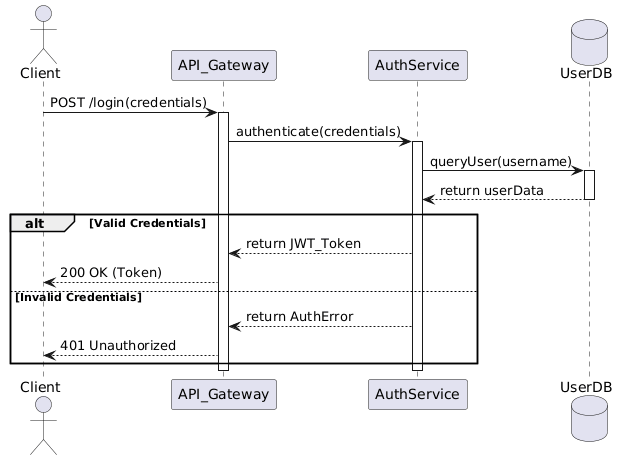
\includegraphics[width=0.85\linewidth]{d4.png}
\\{\small Diagram 4}
\end{center}
What type of message is represented by the dashed arrows returning to the left?
\begin{enumerate}[label=\alph*)]
\item A new method call
\item \ifshowanswers\textbf{A return message with a result}\else A return message with a result\fi
\item An asynchronous broadcast
\item A database update
\end{enumerate}

\item
Review the diagram below.
\begin{center}
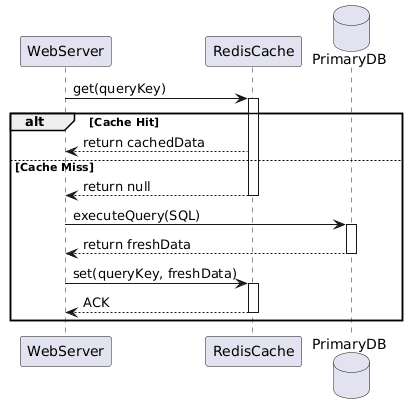
\includegraphics[width=0.85\linewidth]{d5.png}
\\{\small Diagram 5}
\end{center}
Under what specific condition does the sequence diagram show a message being sent to the \texttt{PrimaryDB}?
\begin{enumerate}[label=\alph*)]
\item When the WebServer first starts.
\item Every time a request is made.
\item \ifshowanswers\textbf{Only when a Cache Miss occurs (the data is not in Redis).}\else Only when a Cache Miss occurs (the data is not in Redis).\fi
\item Only when a Cache Hit occurs.
\end{enumerate}

\item
Review the diagram below.
\begin{center}
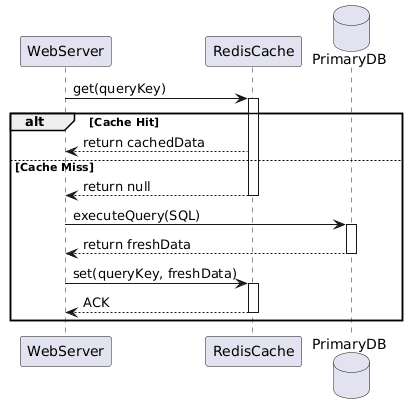
\includegraphics[width=0.85\linewidth]{d5.png}
\\{\small Diagram 5}
\end{center}
What happens immediately after the \texttt{PrimaryDB} returns \texttt{freshData} to the \texttt{WebServer}?
\begin{enumerate}[label=\alph*)]
\item The \texttt{WebServer} sends the data to the client.
\item The \texttt{RedisCache} is cleared.
\item \ifshowanswers\textbf{The \texttt{WebServer} saves the \texttt{freshData} into the \texttt{RedisCache} using a \texttt{set} command.}\else The \texttt{WebServer} saves the \texttt{freshData} into the \texttt{RedisCache} using a \texttt{set} command.\fi
\item The sequence ends.
\end{enumerate}

\item
Review the diagram below.
\begin{center}
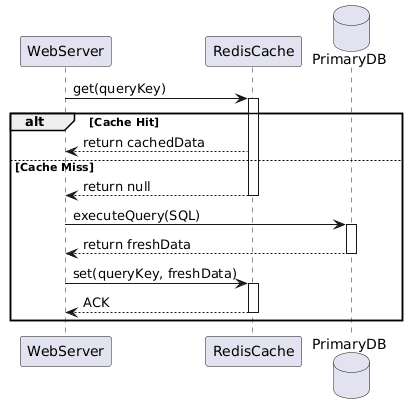
\includegraphics[width=0.85\linewidth]{d5.png}
\\{\small Diagram 5}
\end{center}
What is the primary purpose of a sequence diagram?
\begin{enumerate}[label=\alph*)]
\item \ifshowanswers\textbf{To visualize the order of messages passed between objects over time.}\else To visualize the order of messages passed between objects over time.\fi
\item To show the static relationships and attributes of classes.
\item To display the physical deployment of hardware.
\item To illustrate the state changes of a single object.
\end{enumerate}

\item
Review the diagram below.
\begin{center}
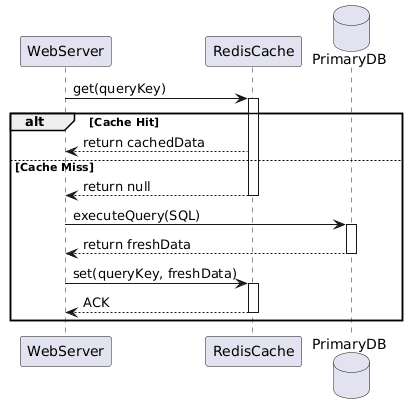
\includegraphics[width=0.85\linewidth]{d5.png}
\\{\small Diagram 5}
\end{center}
Which object initiates the first action in this specific interaction?
\begin{enumerate}[label=\alph*)]
\item RedisCache
\item PrimaryDB
\item \ifshowanswers\textbf{WebServer}\else WebServer\fi
\item The user
\end{enumerate}

\item
Review the diagram below.
\begin{center}
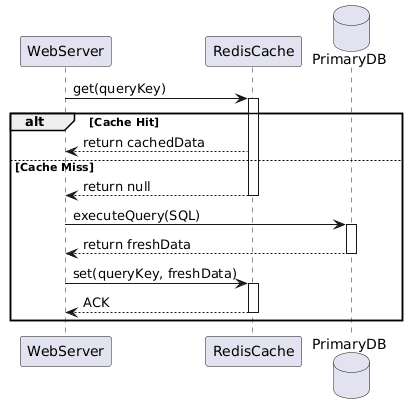
\includegraphics[width=0.85\linewidth]{d5.png}
\\{\small Diagram 5}
\end{center}
What do the vertical dashed lines dropping down from the object names represent?
\begin{enumerate}[label=\alph*)]
\item Data flow constraints
\item \ifshowanswers\textbf{The object's lifeline over time}\else The object's lifeline over time\fi
\item Method signatures
\item Network connections
\end{enumerate}

\item
Review the diagram below.
\begin{center}
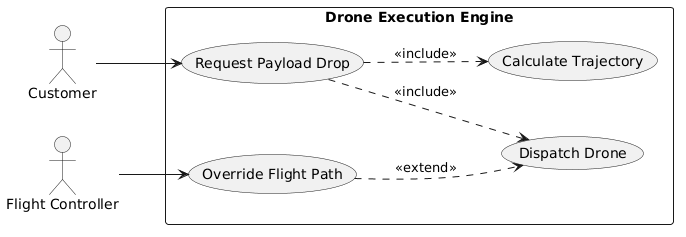
\includegraphics[width=0.85\linewidth]{d6.png}
\\{\small Diagram 6}
\end{center}
What does an \texttt{<<include>>} relationship signify in a use case diagram?
\begin{enumerate}[label=\alph*)]
\item The included use case is optional.
\item \ifshowanswers\textbf{The base use case always requires the execution of the included use case to complete its goal.}\else The base use case always requires the execution of the included use case to complete its goal.\fi
\item The included use case is an alternative error path.
\item The included use case can only be triggered by a system administrator.
\end{enumerate}

\item
Review the diagram below.
\begin{center}
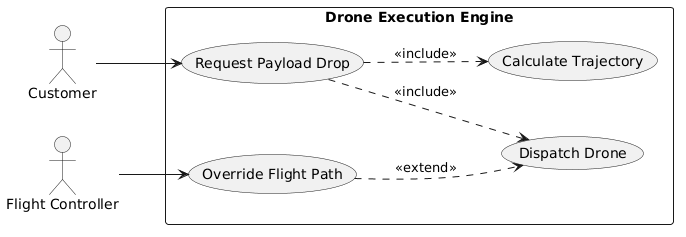
\includegraphics[width=0.85\linewidth]{d6.png}
\\{\small Diagram 6}
\end{center}
How does the \texttt{<<extend>>} relationship differ from the \texttt{<<include>>} relationship?
\begin{enumerate}[label=\alph*)]
\item It is used to show inheritance between actors.
\item It means the base use case must always run the extended use case.
\item \ifshowanswers\textbf{It represents optional or conditional behavior that can be inserted into the base use case.}\else It represents optional or conditional behavior that can be inserted into the base use case.\fi
\item It connects a use case to an external database.
\end{enumerate}

\item
Review the diagram below.
\begin{center}
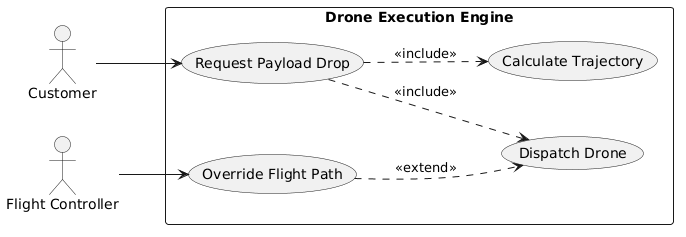
\includegraphics[width=0.85\linewidth]{d6.png}
\\{\small Diagram 6}
\end{center}
What role do the "Customer" and "Flight Controller" figures play in this diagram?
\begin{enumerate}[label=\alph*)]
\item They represent internal software modules.
\item They represent databases.
\item \ifshowanswers\textbf{They represent external actors that interact with the system.}\else They represent external actors that interact with the system.\fi
\item They represent use cases.
\end{enumerate}

\item
Review the diagram below.
\begin{center}
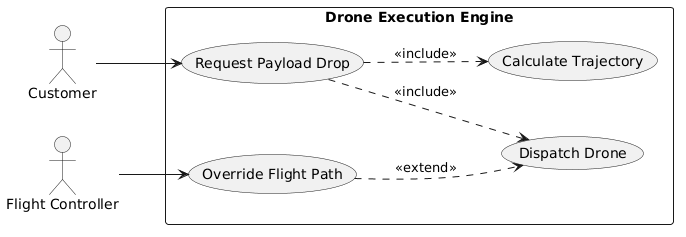
\includegraphics[width=0.85\linewidth]{d6.png}
\\{\small Diagram 6}
\end{center}
Based on the lines connecting actors to use cases, who is allowed to trigger the "Override Flight Path" feature?
\begin{enumerate}[label=\alph*)]
\item The Customer
\item \ifshowanswers\textbf{The Flight Controller}\else The Flight Controller\fi
\item Both the Customer and the Flight Controller
\item The Drone Execution Engine
\end{enumerate}

\item
Review the diagram below.
\begin{center}
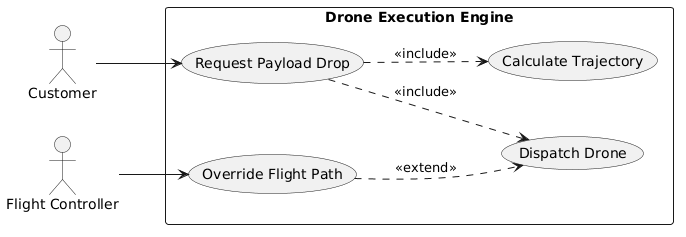
\includegraphics[width=0.85\linewidth]{d6.png}
\\{\small Diagram 6}
\end{center}
What is the purpose of the large rectangle labeled "Drone Execution Engine"?
\begin{enumerate}[label=\alph*)]
\item It represents a hardware server.
\item It shows the timeline of events.
\item \ifshowanswers\textbf{It defines the system boundary, separating internal functionality from external actors.}\else It defines the system boundary, separating internal functionality from external actors.\fi
\item It is a class containing methods and attributes.
\end{enumerate}

\item
Review the diagram below.
\begin{center}
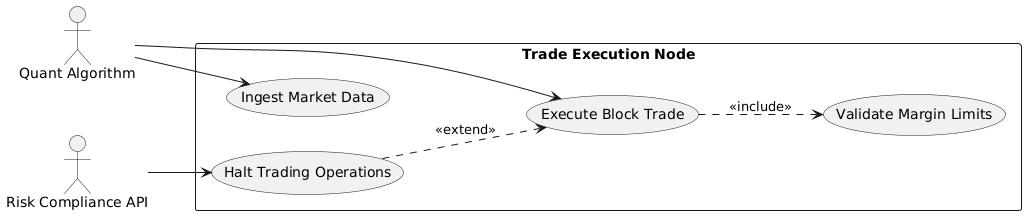
\includegraphics[width=0.85\linewidth]{d7.png}
\\{\small Diagram 7}
\end{center}
Which use cases can the "Quant Algorithm" actor directly initiate?
\begin{enumerate}[label=\alph*)]
\item \ifshowanswers\textbf{Ingest Market Data and Execute Block Trade}\else Ingest Market Data and Execute Block Trade\fi
\item Execute Block Trade and Validate Margin Limits
\item Halt Trading Operations
\item All use cases in the system
\end{enumerate}

\item
Review the diagram below.
\begin{center}
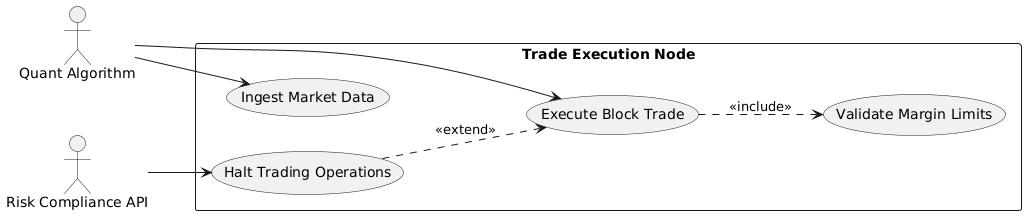
\includegraphics[width=0.85\linewidth]{d7.png}
\\{\small Diagram 7}
\end{center}
Because "Execute Block Trade" has an \texttt{<<include>>} relationship with "Validate Margin Limits", what is true about the execution flow?
\begin{enumerate}[label=\alph*)]
\item Validating limits happens independently of trades.
\item \ifshowanswers\textbf{Every time a block trade is executed, the margin limits must also be validated.}\else Every time a block trade is executed, the margin limits must also be validated.\fi
\item Margin limits are only validated if an error occurs.
\item Validating margin limits is an optional step chosen by the actor.
\end{enumerate}

\item
Review the diagram below.
\begin{center}
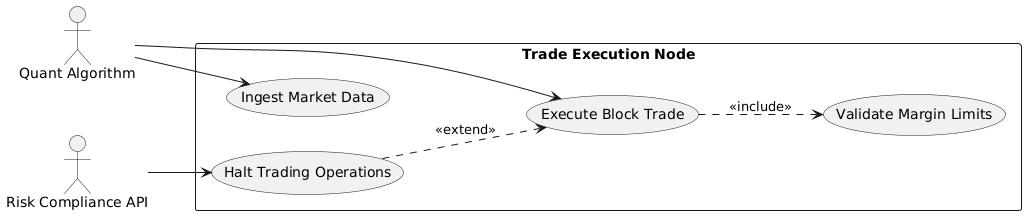
\includegraphics[width=0.85\linewidth]{d7.png}
\\{\small Diagram 7}
\end{center}
If the "Risk Compliance API" decides to trigger "Halt Trading Operations", how does this affect "Execute Block Trade"?
\begin{enumerate}[label=\alph*)]
\item It deletes the trade from the database.
\item It speeds up the trade processing.
\item \ifshowanswers\textbf{It acts as an extension, meaning the halt operation can conditionally interrupt or modify the standard trade execution.}\else It acts as an extension, meaning the halt operation can conditionally interrupt or modify the standard trade execution.\fi
\item It converts the trade into market data.
\end{enumerate}

\item
Review the diagram below.
\begin{center}
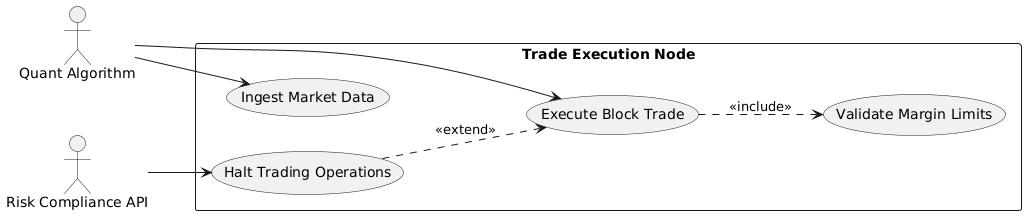
\includegraphics[width=0.85\linewidth]{d7.png}
\\{\small Diagram 7}
\end{center}
Can the "Risk Compliance API" directly trigger the "Ingest Market Data" use case?
\begin{enumerate}[label=\alph*)]
\item Yes, because it is an actor.
\item \ifshowanswers\textbf{No, there is no association line connecting them.}\else No, there is no association line connecting them.\fi
\item Yes, through the extend relationship.
\item Only if the Quant Algorithm fails.
\end{enumerate}

\item
Review the diagram below.
\begin{center}
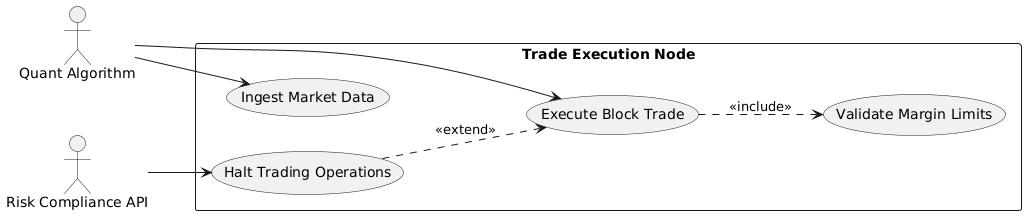
\includegraphics[width=0.85\linewidth]{d7.png}
\\{\small Diagram 7}
\end{center}
In object-oriented analysis, what is the primary goal of creating a use case diagram?
\begin{enumerate}[label=\alph*)]
\item To write the actual source code for the software.
\item To plan the database schema and tables.
\item \ifshowanswers\textbf{To capture the functional requirements of the system from the user's perspective.}\else To capture the functional requirements of the system from the user's perspective.\fi
\item To define the exact order of method calls.
\end{enumerate}

\end{enumerate}


\ifshowanswers
\section*{Answer Key}
\begin{enumerate}[leftmargin=*, label=\textbf{\arabic*.}]
\item b
\item b
\item b
\item c
\item a
\item b
\item b
\item b
\item c
\item d
\item c
\item c
\item b
\item a
\item c
\item a
\item b
\item c
\item c
\item b
\item c
\item c
\item a
\item c
\item b
\item b
\item c
\item c
\item b
\item c
\item a
\item b
\item c
\item b
\item c
\end{enumerate}
\fi

\end{document}
